\documentclass[oneside]{book}
\usepackage{setspace}
\usepackage{hyperref}
\usepackage{fancyhdr}
\pagestyle{fancyplain}
\fancyhf{}
\fancyfoot[c]{\thepage}
\renewcommand{\headrulewidth}{0pt}
\usepackage{graphicx}
\usepackage{xepersian}
\settextfont{XB Yas}


\title{گزارش سامانه بوستان}
\author{نیلوفر علیخانی\\رومینا رئوفیان\\شیما باقریان\\امیر حسین صفدریان\\احسان جلالی\\علی ماهوش\\ 
	\\دکتر بهمن زمانی}

\begin{document}

	
\begin{figure}[h!]	
\begin{center}

\includegraphics[height = 4cm,width= 4cm]{University of Isfahan.jpg}
\\
دانشگاه اصفهان\\
دانشکده کامپیوتر\\
گروه آموزشی نرم افزار\\
\end{center}
\maketitle
\end{figure}


\newpage
\doublespacing
\tableofcontents
\newpage
\chapter{فصل اول:مقدمه}
\newpage
\section{معرفی سامانه}

\large
این پروژه، یک سیستم نرم افزاری است که هدف آن کمک به دانشجویان و افزایش نظم  انتخاب واحد، آسان‌تر شدن انتخاب واحد برای دانشجو هم چنین کمک به مسئولین آموزش برای برنامه ریزی بهتر می‌باشد.  

 این سامانه «بوستان» نام دارد که با دریافت ملزومات انتخاب واحد مانند لیست و مشخصات دروس ارائه شده، معدل دانشجو، چارت درسی و از این دست موارد مورد نیاز و نیز با استفاده از چارت و دروس گذرانده شده، به دانشجو در انتخاب دروس کمک می کند و در نهایت تعدادی برنامه ی هفتگی مناسب با شرایط ذکر شده در بالا برای انتخاب ارائه دهد.
 
 یکی دیگر از قابلیت های این سیستم  ایجاد کردن چند برنامه هفتگی با رعایت پیشنیاز ها و هم نیاز های دروس مربوطه، پرسش و پاسخ و تعامل با معاون آموزشی و هم چنین نمایش نحوه ارزیابی اساتید اشاره کرد.
 
 این سیستم با دانشجو نیز تعامل مناسبی دارد به این شکل که با در اختیار قرار دادن امکاناتی همچون: نمایش تعداد متقاضیان هر درس، حضور و یا عدم حضور دوستان وی در آن کلاس، ساعاتی که ترجیح او است که کلاس داشته باشد، اساتیدی که از روی علاقه می‌خواهد با آن ها کلاس داشته باشد و مواردی از این دسته که این مسئله را بیان می کند: دانشجو می تواند برنامه درسی مطلوب خود را برحسب فیلتر های اعمال شده دریافت کند.
 
  
\newpage
\section{ارتباط با سامانه‌های دیگر}

\begin{figure}[h!]
	
	
طبق چارت سازمانی دانشگاه اصفهان و زیرسیستم های موجود و وظایفشان، بوستان زیرسیستم «مدیریت امور آموزشی» است که خود آن  زیرسیستم «معاونت آموزشی و تحصیلات تکمیلی» به حساب می‌آید و در نمودار چارت سازمانی در کنار زیر سیستم هایی چون «امور پذیرش و ثبت نام و خدمات»، «خدمات رایانه ای» و «اداره دانش آموختگان» قرار دارد.

	
\begin{center}
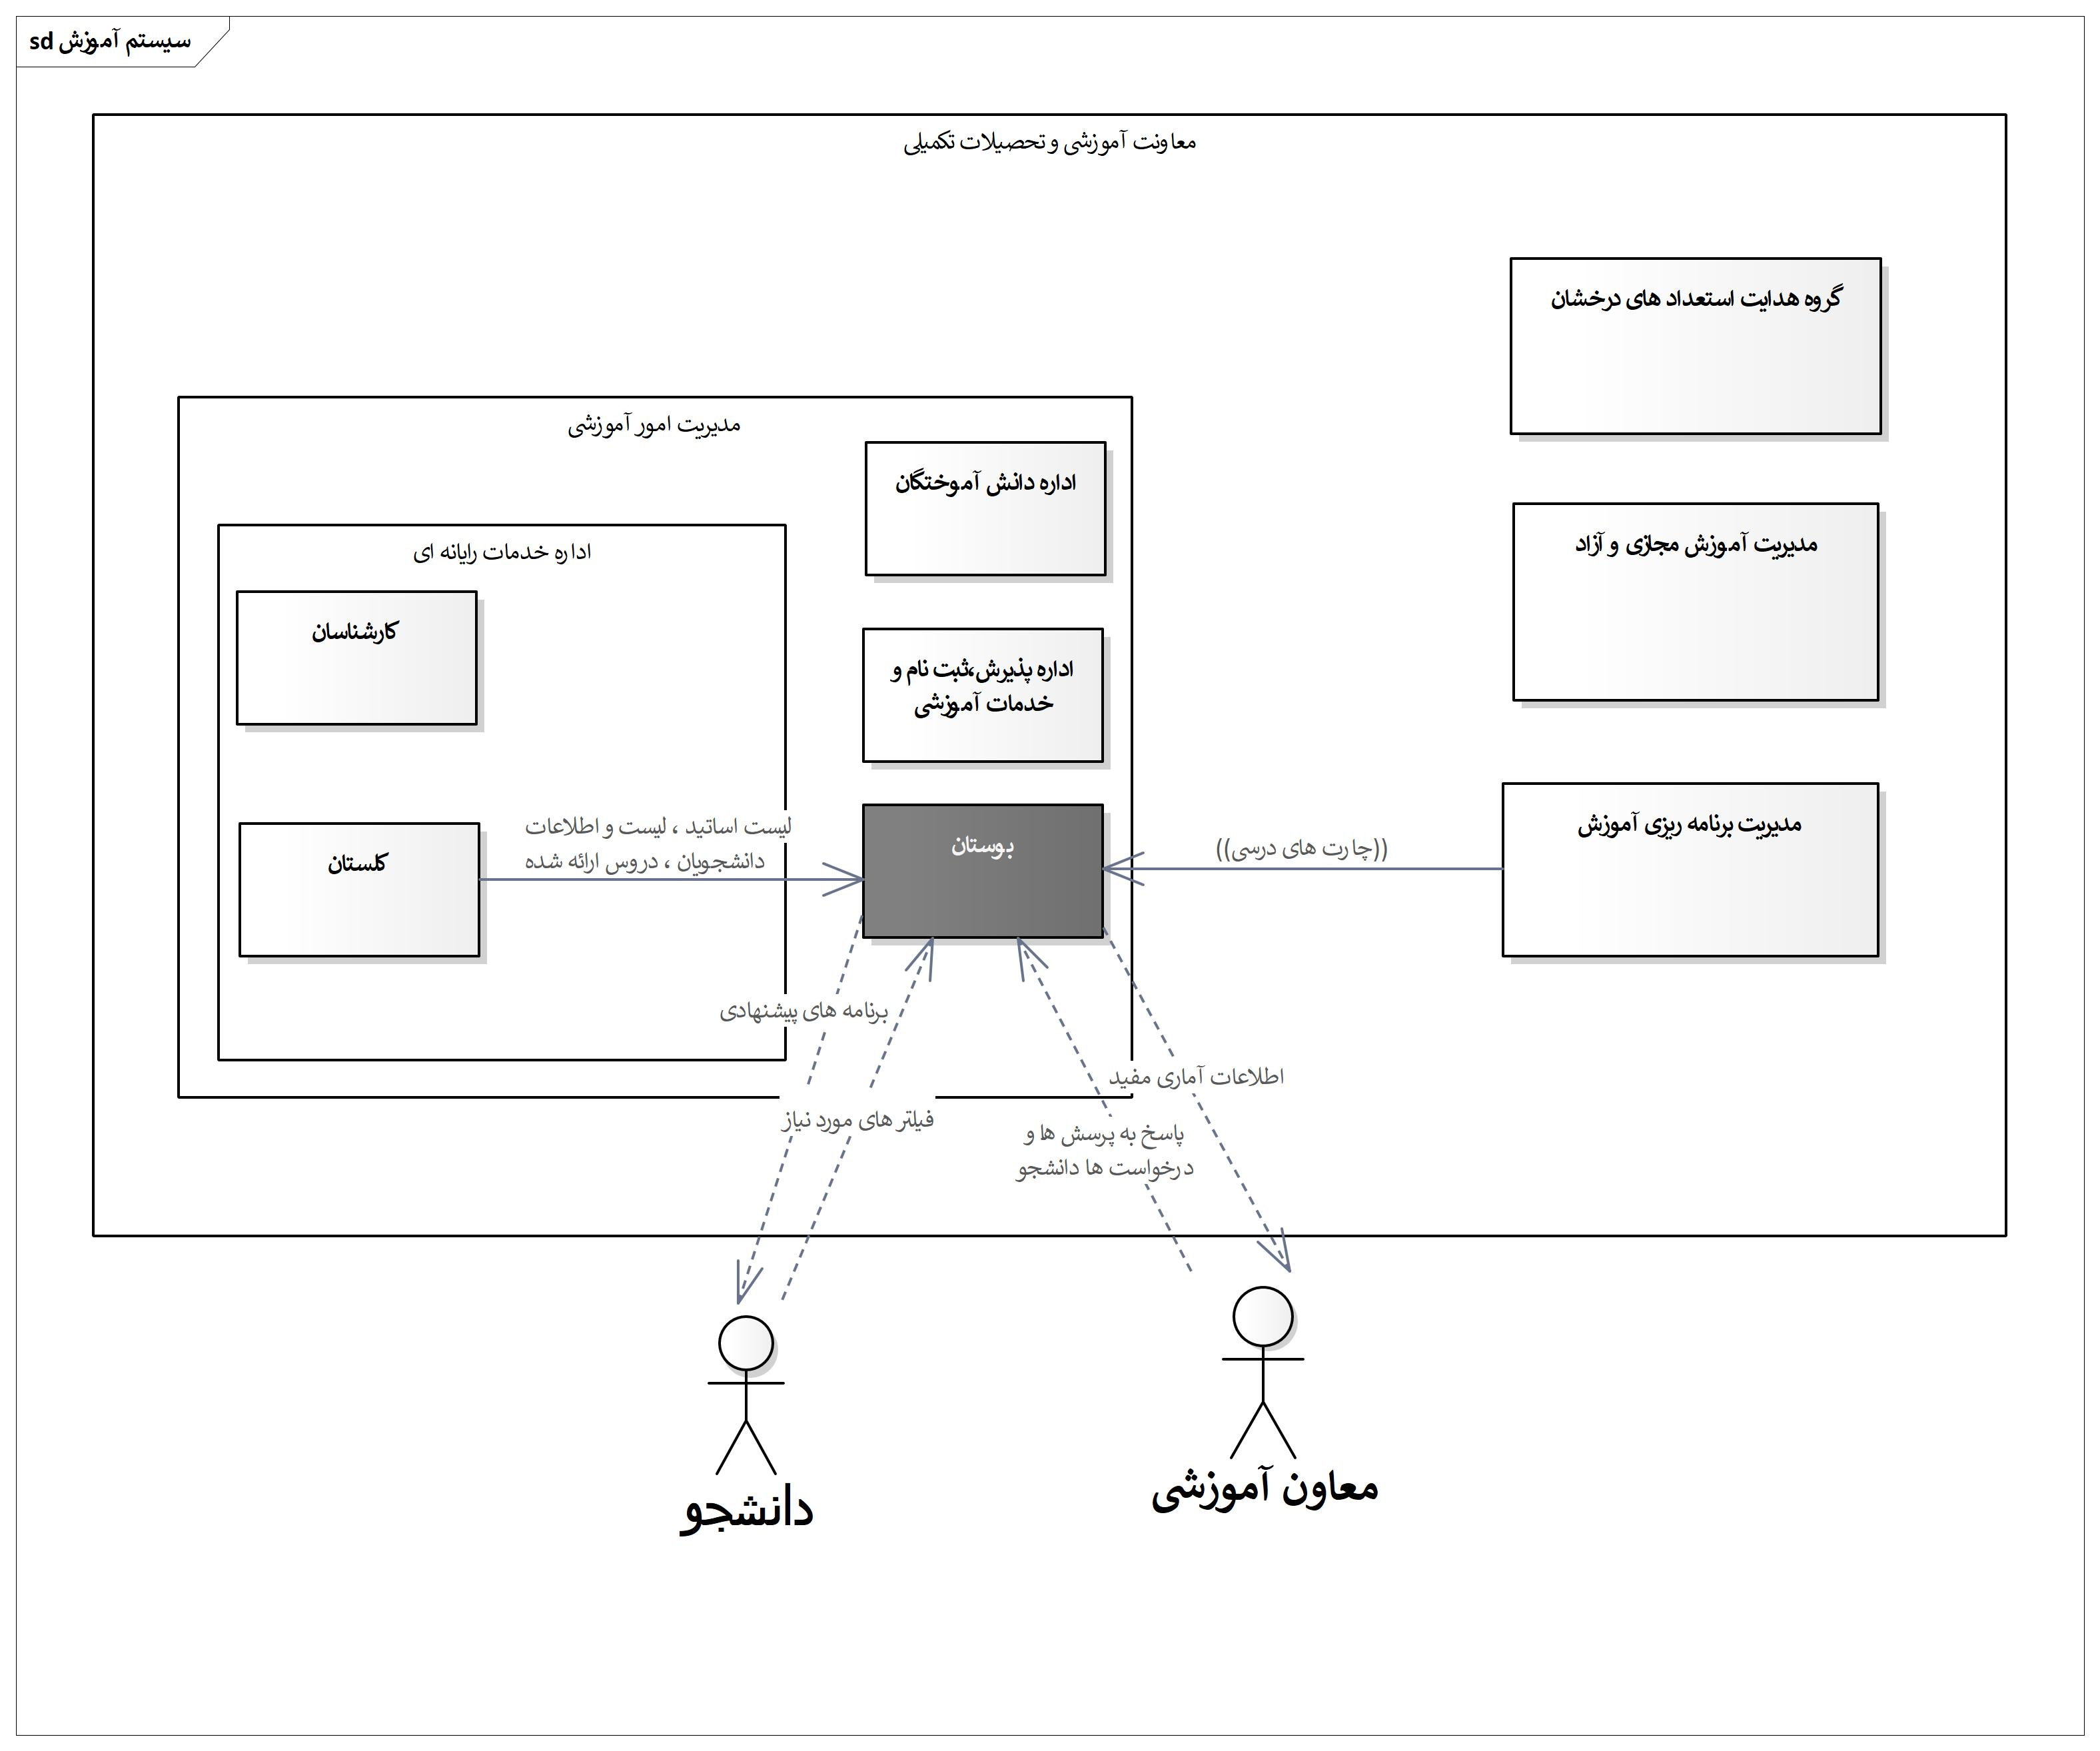
\includegraphics[height = 12cm,width= 10cm]{Education system.jpg}	\begin{center}
\caption{نمودار بلوکی برای سیستم بوستان در آموزش}
\end{center}
		
\end{center}
\end{figure}
 
\newpage
 
 این سامانه برای انجام وظایف خود نیاز به ارتباط و تبادل با زیرسیستم های دیگر نیز دارد.
 
 در سیستم آموزش دانشگاه، وظیفه ی رسیدگی به امور آموزشی بر عهده ی سیستم «معاونت آموزشی و تحصیلات تکمیلی» می باشد که سیاست گذاری برنامه های آموزشی و درسی دانشگاه برعهده ی زیرسیستم «مدیریت برنامه ریزی آموزشی» می باشد و وظیفه ی رسیدگی و اجرای این سیاست ها بر عهده ی سیستم «مدیریت امور آموزشی» می باشد و از آنجا که وظیفه ی سیستم بوستان کمک به اجرای همین سیاست ها می‌باشد، پس بخشی از سیستم «مدیریت امور آموزشی» است.
 
 
 همان‌طور که در بالا نیز اشاره شد سیستم «مدیریت امور آموزشی» خود از زیرسیستم های «اداره خدمات رایانه ای»، «اداره پذیرش، ثبت نام و خدمات آموزشی» و «اداره دانش آموختگان» تشکیل شده است. از بین این زیرسیستم ها، وظیفه ی رسیدگی به امور انتخاب واحد و ارائه ی دروس در هر ترم در سامانه ی گلستان برعهده ی «اداره خدمات رایانه ای» می‌باشد.
 
 از آنجا که سامانه ی بوستان برای انجام انتخاب واحد نقشی کمک کننده به سامانه ی گلستان خواهد داشت  و با توجه به تعاملات آن با این سیستم می‌توان نتیجه گرفت که سیستم بوستان نمی‌تواند زیرسیستم بخش «اداره خدمات رایانه ای» باشد.
 
  مشخص کردن چارت درسی یکی از وظایف سیستم «مدیریت برنامه ریزی آموزشی» است و سامانه ی بوستان برای عمل کردن به چارت درسی به آن نیاز دارد بنابراین سامانه ی بوستان چارت آموزشی و قوانین آن را از سیستم «مدیریت برنامه ریزی آموزشی» دریافت می کند.
  
  نگهداری اطلاعات مربوط به دانشجو وظیفه ی «اداره خدمات رایانه ای» می باشد که این کار توسط سامانه گلستان انجام می شود. اما ربط آن به سامانه ی بوستان این است که این سامانه  باید معدل، تعداد ترم گذراند شده، دروس افتاده، پاس شده و گذرانده ی دانشجو را از قسمت اطلاعات جامع دانشجو سامانه ی گلستان و به عبارتی دیگر از سیستم «اداره خدمات رایانه ای» دریافت کند.
  
  جمع آوری دروس هر ترم از دانشکده هایی که آن دروس را ارائه داده اند وظیفه ی «ارائه خدمات رایانه ای» از سیستم «مدیریت امور آموزشی» است که این کار توسط سامانه گلستان انجام می شود بنابراین سامانه ی بوستان باید دروس ارائه شده ی هر ترم را همراه با ساعات ارائه شده و ظرفیت و اساتید آن را از قسمت گزارش های آموزشی سامانه ی گلستان و درواقع از سیستم «ارائه خدمات رایانه ای» دریافت کند.
 
 

\end{document}